%% start of file `template.tex'.
%% Copyright 2006-2013 Xavier Danaux (xdanaux@gmail.com).
%
% This work may be distributed and/or modified under the
% conditions of the LaTeX Project Public License version 1.3c,
% available at http://www.latex-project.org/lppl/.


\documentclass[11pt,a4paper,sans]{moderncv}        % possible options include font size ('10pt', '11pt' and '12pt'), paper size ('a4paper', 'letterpaper', 'a5paper', 'legalpaper', 'executivepaper' and 'landscape') and font family ('sans' and 'roman')

% modern themes
\moderncvstyle{banking}                            % style options are 'casual' (default), 'classic', 'oldstyle' and 'banking'
\moderncvcolor{red}                                % color options 'blue' (default), 'orange', 'green', 'red', 'purple', 'grey' and 'black'
%\renewcommand{\familydefault}{\sfdefault}         % to set the default font; use '\sfdefault' for the default sans serif font, '\rmdefault' for the default roman one, or any tex font name
%\nopagenumbers{}                                  % uncomment to suppress automatic page numbering for CVs longer than one page

% character encoding
\usepackage[utf8]{inputenc}                       % if you are not using xelatex ou lualatex, replace by the encoding you are using
%\usepackage{CJKutf8}                              % if you need to use CJK to typeset your resume in Chinese, Japanese or Korean

% adjust the page margins
\usepackage[scale=0.75]{geometry}
%\setlength{\hintscolumnwidth}{3cm}                % if you want to change the width of the column with the dates
%\setlength{\makecvtitlenamewidth}{10cm}           % for the 'classic' style, if you want to force the width allocated to your name and avoid line breaks. be careful though, the length is normally calculated to avoid any overlap with your personal info; use this at your own typographical risks...

\usepackage{graphicx}
\usepackage{import}

% personal data
\name{Mydul}{Islam}
\title{Curriculum Vitae}                               % optional, remove / comment the line if not wanted
\address{17/A-12, 1 No Road, Mehedibug Housing, Adabor, Shyamoli, Dhaka-1207}{}{}% optional, remove / comment the line if not wanted; the "postcode city" and and "country" arguments can be omitted or provided empty
\phone[mobile]{+88 01712 821277}                   % optional, remove / comment the line if not wanted
\phone[fixed]{+88 01680 403000}                    % optional, remove / comment the line if not wanted
%\phone[fax]{+3~(456)~789~012}                      % optional, remove / comment the line if not wanted
\email{muhurtoo@gmail.com}                               % optional, remove / comment the line if not wanted
\homepage{www.about.me/mydul}                         % optional, remove / comment the line if not wanted
%\extrainfo{additional information}                 % optional, remove / comment the line if not wanted
%\photo[64pt][0.4pt]{picture}                       % optional, remove / comment the line if not wanted; '64pt' is the height the picture must be resized to, 0.4pt is the thickness of the frame around it (put it to 0pt for no frame) and 'picture' is the name of the picture file
%\quote{Some quote}                                 % optional, remove / comment the line if not wanted

% to show numerical labels in the bibliography (default is to show no labels); only useful if you make citations in your resume
%\makeatletter
%\renewcommand*{\bibliographyitemlabel}{\@biblabel{\arabic{enumiv}}}
%\makeatother
%\renewcommand*{\bibliographyitemlabel}{[\arabic{enumiv}]}% CONSIDER REPLACING THE ABOVE BY THIS

% bibliography with mutiple entries
%\usepackage{multibib}
%\newcites{book,misc}{{Books},{Others}}

%----------------------------------------------------------------------------------
%            content
%----------------------------------------------------------------------------------
\begin{document}
%\begin{CJK*}{UTF8}{gbsn}                          % to typeset your resume in Chinese using CJK

%----------------------------------------------------------------------------------------
%	COVER LETTER
%----------------------------------------------------------------------------------------

% To remove the cover letter, comment out this entire block

\clearpage

\recipient{HR Departmnet}{Google Inc.\\123 Pleasant Lane\\Silicon Vali, California} % Letter recipient
\date{\today} % Letter date
\opening{Dear Hiring Manager,} % Opening greeting
\closing{Sincerely yours,\\ 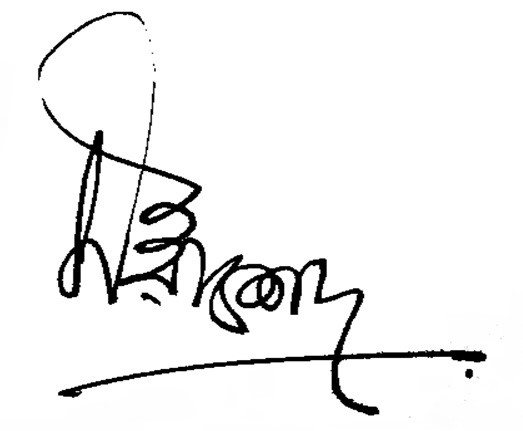
\includegraphics[width=0.2\linewidth]{signature.jpg}} % Closing phrase
\enclosure[Acknowledgements:]{This Cover letter and CV are created by using LaTex{}} % List of enclosed documents

\makelettertitle % Print letter title

I am writing to express my interest in your posting on "bdjobs.com" for an Electrical and Electronic Engineer (EEE). After reading the job description I am confident that I would be a perfect fit for this position because of my thinking abilities, knowledge and skills. I love to work with different platform and I always try to do new experiment. 

Now i am running two research parallelly. I worked with Artificial Intelligence, Embedded System, Robotics. One of my research have been published recently in EEE Annual Journal which is about "Arithmetic Logic Unit (ALU)". Now I am working with CMOS Double Gate IC designing.

I enjoy solving logical operation, fixing hardware and programming problems, and feel a sense of accomplishment when a solution is determined and built. I love challenges and I always try to work with new technologies. I believe your company will be the best place for me to apply my education and working knowledge.
Therefore, I would welcome the chance of an interview, where we would be able to discuss in greater detail the value and strength I can bring to your already successful company.

I’ve attached a copy of my resume that details my experience, educational background, research works, projects, achievements and my interested fields.
Thank you for your time and consideration. I look forward to speaking with you about this employment opportunity.

\vspace{0.5cm}

\makeletterclosing % Print letter signature

%----------------------------------------------------------------------------------------

%-----       resume       ---------------------------------------------------------
\clearpage
\makecvtitle

\small{Electrical and Electronic Engineer who completed the bachelor's degree and too busy to spend time doing research. Passionate about science, with strong technical, business, and interpersonal skills for working in a team and successfully completing a project.}

\section{Previous Employment}

\vspace{6pt}

\begin{itemize}

\item{\cventry{Jan 2016 -- Dec 2016}{Part time Assistant Engineer}{Power Engineers BD}{Dhaka}{}{\vspace{3pt}I was responsible for the administrative duties and the tidiness and general order of the Company. I worked in a safety-oriented manner, often working alongside construction and servicing machinery. At the end of my work with the company my colleagues praised my work ethic.}}

\vspace{6pt}

\item{\cventry{Oct 2013 -- Present}{CEO and Founder}{Icche Creation}{Dhaka}{}{\vspace{3pt}I worked for more then three years as a team leader to maintaining this Start-up and providing new idea for co-workers. I was often trusted with each other jobs but i wanna do something different. As a founder and team leader I would delegate tasks to a team of about 5 people, often new staff who needed training, and lead the group to service. During this time I worked in a highly professional manner and was focused to provide excellent customer service.}}

\vspace{6pt}

\item{\cventry{2013 -- 2015}{Contributor/Writer}{The Daily Janakantha}{Dhaka}{}{\vspace{3pt}I spent near about three years as a Weekly Contributor Writer on Entertainment Page of this daily Newspaper for some work experience in Journalism field. My roles included writing article, Visiting and collecting raw materials from media, Page makeup and Interviewing various public figure.}}

\vspace{6pt}

\item{\cventry{Mar 2012 -- Oct 2015}{Freelance Web Designer}{Upwork (Odesk)}{Dhaka}{}{\vspace{3pt}Including me every man want freedom, even within job life. At that view many people choose Freelancing. I was spent a huge time for working as a Web Designer and Developer. Somehow i was detached and i was switched from this field.}}

\end{itemize}

\newpage

\section{Education}

\vspace{5pt}

\subsection{Academic Qualifications}

\vspace{5pt}

\begin{itemize}

\item{\cventry{2012--2015}{B.Sc.(Hons) Electrical and Electronic Engineering }{Daffodil International University}{Dhaka}{\textit{Major: Electronics and Minor: Power}}{}}

\item{\cventry{2010}{HSC}{Bhola Government University College}{Bhola Sadar, Barishal}{\textit{Science}}{}}  % arguments 3 to 6 can be left empty

\item{\cventry{2008}{SSC}{Daori Hat Secondary School}{Daori Bazar, Lalmohan, Bhola}{\textit{Science}}{}}

\end{itemize}

\vspace{2pt}

\subsection{Notable Projects}

\vspace{5pt}

\begin{itemize}

\item{\textbf{Bachelors Project (Ongoing):} \textit{'CMOS VLSI Design'}

\vspace{3pt}

\small{Complementary metal oxide semiconductor, abbreviated as CMOS 'si:mos', is a technology for constructing integrated circuits. CMOS also allows a high density of logic functions on a chip. It was primarily for this reason that CMOS became the most used technology to be implemented in VLSI chips.}}

\vspace{6pt}

\item{\textbf{3rd year Individual Project:} \textit{'Arithmetic Logic Unit (ALU)'}

\vspace{3pt}

\small{An arithmetic logic unit (ALU) is a digital circuit used to perform arithmetic and logic operations. It represents the fundamental building block of the central processing unit (CPU) of a computer. Modern CPUs contain very powerful and complex ALUs. In addition to ALUs, modern CPUs contain a control unit (CU).}}

\vspace{6pt}

\item{\textbf{Annual Inter-University EEE Project Exhibition:} \textit{'Quad-Copter (Drone); MFROBO 1501'}

\vspace{3pt}

\small{A Quad-copter, also called a Quadrotor helicopter or quadrotor, is a multirotor helicopter that is lifted and propelled by four rotors. Quadcopters are classified as rotorcraft, as opposed to fixed-wing aircraft, because their lift is generated by a set of rotors (vertically oriented propellers).
Quadcopter designs also became popular in unmanned aerial vehicle (UAV or drone) research. With their small size and maneuverability, these quadcopters can be flown indoors as well as outdoors.}}

\vspace{6pt}

\item{\textbf{EEE Day 2016:} \textit{'Android Based Obstacle Detector Car Robot'}

\vspace{3pt}

\small{Now day’s many industries are using robots due to their high level of performance and reliability and which is a great help for human beings. The obstacle avoidance robotics is used for detecting obstacles and avoiding the collision. This is an autonomous robot.
The robot gets the information from surrounding area through mounted sensors on the robot. Some sensing devices used for obstacle detection like bump sensor, infrared sensor, ultrasonic sensor etc. It is low cost and it has high ranging capability.}}

\vspace{6pt}

\item{\textbf{Individual Lab project:} \textit{'DIY: Center Tap STEP-DOWN Transformer'}

\vspace{3pt}

\small{It converts 220 volts into 35 or 12 volts. It is useful for any kind of load which requires 35 or 12 volts. Besides various amplifications are possible with it. It is more efficient from others ready-made Transformer.}}

\vspace{6pt}

\item{\textbf{Social welfare work:} \textit{'Web For Society'}

\vspace{3pt}

\small{During the college life i spent a week completing a public project for Social welfare. It was totally free for society. I worked with a team operating as consultants for some particular problem the rural people was having. During this project I was working in a professional environment, and co-operating with various managers and engineers to create a design that met the requirements of the problem.}}

\end{itemize}

\newpage

\subsection{Notable Publications}

\vspace{5pt}

\begin{itemize}

\item{\textbf{Smart Security System Through Password Protected Smart Control System of Home Appliance} \textit{\\-EEE Annual Journal 2016}

\vspace{3pt}

\small{In this Work, Presents the development of GSM-based home appliance control for smart home system. The main aim of the prototype development is to reduce electricity wastage.
GSM module is used for receiving  short message  service (SMS) from user’s mobile phone  that automatically enable the controller to take any further action such as to switch ON and OFF the home appliances such as light, air-conditioner, fan, water pump, door, TV etc. The system is integrated with Arduino and GSM network interface using a programming language which is the combination of C language.
The prototype has been successfully developed and it could provide an effective mechanism in utilizing the energy source efficiently.}}

\vspace{6pt}

\item{\textbf{Analysis, Design and Simulation of Arithmetic Logic Unit (ALU) by basic gates} \textit{\\-EEE Annual Journal 2015}

\vspace{3pt}

\small{The paper shows the Arithmetic Logic Unit (ALU) is a digital electronic circuit that performs arithmetic and bitwise logical operations on integer binary numbers. This is in contrast to a floating-point unit (FPU), which operates on floating point numbers. An ALU is a fundamental building block of many types of computing circuits, including the central processing unit (CPU) of computers.}}

\vspace{6pt}

\item{\textbf{Book: "Operation Pure Hashi"} \textit{\\-Ekushey Book Fair-2013}

\vspace{3pt}

\small{A great delightful story set in a delightful mix of writers. I love to Read and I love to write. Poetry is the on of my most favorite things. But one day i decide to write a book for smile means entertaing people by story. But its the tough things in literature. But i tried again again with keyboard and finally i wrote a book with full delightful story. It's not only for kids but all ages people who love to lough.}}

\end{itemize}

\section{Technical and Personal skills}

\vspace{6pt}

\begin{itemize}

\item \textbf{Programming and Scripting Languages:} Proficient in: C, Python, Matlab, Arduino, LaTeX \\ HTML5, CSS3, Git. Also basic ability with: Assembly, Micro controller, VBA, VHDL.

\vspace{6pt}

\item \textbf{Industry Software Skills:} Cadence (Intermediate), Micro-wind (Advanced), Matlab R2016b (Advanced), Pspice (Intermediate), LTspice (Intermediate), Auto-cad (Intermediate), Proteus (Advanced), \\COMSOL Multiphysics (Basic), Adobe Photo-shop CS6 (Basic), Most MS Office products including MS project and MS access (Advanced).

\vspace{6pt}

\item \textbf{Accustomed to the environment:} Mac OS,\\ Linux (Ubuntu, Mint, Debian, Fedora, Red hat, Kali), \\ Windows (Xp, 7, 8, 10).

\vspace{6pt}

\item \textbf{General Business Skills:} Good presentation skills, Works well in a team.

\vspace{6pt}

\item \textbf{Other:} Good soldering and spot welding skills, Can write well organized and structured reports.

\end{itemize}

\section{Achievement}

\vspace{6pt}

\begin{itemize}

\item \textbf{Certification for Project Showcasing Competition:} 'Inter University Championship' \\ EEE-PW16-002 (Dec 2016)

\vspace{6pt}

\item \textbf{National Book Reading Competition 2015:} 'British Council' \\ (Oct 2015)

\vspace{6pt}

\item \textbf{Arduino Based Robotics Contests:} 'Pi Labs Bangladesh Ltd' \\ TSB-RW-1504-05 (Mar 2015)

\vspace{6pt}

\item \textbf{AutoCad 3D Designing (Electrical Drawing):} 'Daffodil International University' \\ EEE/FL2014/SCAC/12 (Jan 2015)

\vspace{6pt}

\item \textbf{Dean Certificate Award:} 'Daffodil International University'\\(2015)

\vspace{6pt}

\item \textbf{COMSOL Multiphysics Certifications:} 'Green'\\ WCM35 (December 2014)

\vspace{6pt}

\item \textbf{Inter Collegiate Debate Competition:} 'District Education Office'\\ (2009)

\vspace{6pt}

\item \textbf{General Computer Skills Certification:} 'Rural Incorporate Development Association (RIDA)'\\191/04-195 (2008)

\vspace{6pt}

\item \textbf{Primary School Scholarship:} 'Education Ministry of the People's Republic of Bangladesh Government'\\(2003)

\end{itemize}

\section{Voluntary Work Experiences}

\vspace{6pt}

\begin{itemize}

\item{\textbf{"IEEE"} \textit{Member And Volunteer (Jan 2017) \\ Science And technology}

\vspace{3pt}

\small{The Institute of Electrical and Electronics Engineers (IEEE, pronounced "I triple E") is a professional association with its corporate office in New York City and its operations center in Piscataway, New Jersey.
It was formed in 1963 from the amalgamation of the American Institute of Electrical Engineers and the Institute of Radio Engineers.
Today, it is the world's largest association of technical professionals with more than 400,000 members in chapters around the world.
Its objectives are the educational and technical advancement of electrical and electronic engineering, telecommunications, computer engineering and allied disciplines.}}

\vspace{6pt}

\item{\textbf{"EMK Center"} \textit{Member And Volunteer (Oct 2016) \\ Social Service}

\vspace{3pt}

\small{Edward M. Kennedy (EMK) Center for Public Service and the Arts engages, inspires, connects, and empowers citizens of all ages.

Created in 2012 through a partnership between the Liberation War Museum and the American Center of U.S. Embassy Dhaka, the EMK Center is a non-partisan platform committed to open dialogue, informed action, individual and artistic expression, and personal and professional development. We define public service as service on behalf of the people – by anyone, anywhere, anytime.

The EMK Center honors the legacy of public servants worldwide, exemplified by the men and women who fought for Bangladesh’s independence in 1971 and by U.S. Senator Edward M. Kennedy, who was moved to take action then and throughout his life in support of his convictions. In February 1972, Senator Kennedy planted a banyan tree on Dhaka University’s campus as a living tribute to friendship, resilience, and hope. It stands today.}}

\vspace{6pt}

\item{\textbf{"The Linux Foundation"} \textit{Volunteer (Jun 2016) \\ Science And technology}

\vspace{3pt}

\small{The Linux Foundation is a non-profit technology trade association chartered to promote, protect and advance Linux and collaborative development.}}

\vspace{6pt}

\item{\textbf{"World Literary Center"} \textit{Organizer and Volunteer (Feb 2015)\\ Arts And Culture}

\vspace{3pt}

\small{Bishwo Shahitto Kendro (World-Literature Centre), has been relentlessly working in this direction in an informal way to build a knowledgeable, enriched and committed generation through various intellectual and cultural program since its inception in 1978. 

The principal objective of Bishwo Shahitto Kendro is to create a favorable environment throughout the country for nurturing enlightened individuals, organizing them into a national force and catalyzing enlightenment in the collective persona of the citizens of Bangladesh.}}

\vspace{6pt}

\item{\textbf{"WaterAid"} \textit{Volunteer (Mar 2006)\\ Environment}

\vspace{3pt}

\small{WaterAid has been operating in Bangladesh since 1986 as one of the lead actors in Water, Sanitation and Hygiene (WASH) sector and is well experienced in innovating, scaling up and managing large scale projects targeting poor, vulnerable and excluded.}}

\end{itemize}


\section{Language}

\vspace{6pt}

\begin{itemize}

\item \textbf{English:} Full professional proficiency

\vspace{6pt}

\item \textbf{Bangla:} Native or bilingual proficiency

\end{itemize}

\section{Interests and extra-curricular activity}

\vspace{6pt}

\begin{itemize}

\item{I was a "fresher representative" in my 2nd and 3rd years of university, this required me to guide, look after, and ensure that a particular flat of first years have a good time in their first week, and feel consoled in what for most of them is there first time living away from home. We were responsible for the safety and well being of the group of first years during the first week, and during this time I made good friends with all of them.}

\vspace{6pt}

\item{I am a member of a number of university societies. I was also the vice president of the EEE club and co-founder of the Cultural Society. My roles in this included recruiting members, in which during "fresher's fair" we enlisted over 200 new members. This was regarded as very successful, considering other societies averaged around 50. I also appeared in an interview on the university television station, set up a society bank account, and helped organise the events. One of these events was featured in the local newspaper.}

\vspace{6pt}

\item{I am also an avid hiker, having completed the national 3 peaks challenge last summer. Other interest include guitar, which I am self-taught, and home brewing.}

\vspace{6pt}

\item{I am a crazy fan of the Rubik's Cube and other twisty puzzles. At least each any weekend of a month i will try to join with the unofficial meet-up of the fastest speed-cubers of my country.
My record for a single solve of the 3X3X3 in unofficial competition is 30 seconds.}

\vspace{6pt}

\item{I am a amateur writer. I love to writing poem. My hobby is write something unconsciously which are hard to get, but sometime its be look like as poem. Without any preparation, once upon a day I published a book at Bengali Book Fair "Ekushe Boi mela" 2013 which name is “Operation Pure Smile”. Sometime i wrote poem for publishing to Newspaper, Magazine or Social blog.}

\end{itemize}

\section{References}

\vspace{6pt}
 
\begin{itemize}

\item \textbf{Professor Dr. Md. Quamrul Ahsan} \\Professor And Advisor\\ Ph.D, University of   Ottawa, Canada.\\ Daffodil International University, Bangladesh\\advisor.eee@daffodil.edu.bd

\vspace{10pt}

\item \textbf{Professor. Dr. Md. Fayzur Rahman} \\Professor And Din\\ Ph.D. from Yeungnam University, South Korea. \\Daffodil International University, Bangladesh\\chairman.eee@daffodil.edu.bd

\end{itemize}

% Publications from a BibTeX file without multibib
%  for numerical labels: \renewcommand{\bibliographyitemlabel}{\@biblabel{\arabic{enumiv}}}% CONSIDER MERGING WITH PREAMBLE PART
%  to redefine the heading string ("Publications"): \renewcommand{\refname}{Articles}
\nocite{*}
\bibliographystyle{plain}
\bibliography{publications}                        % 'publications' is the name of a BibTeX file

% Publications from a BibTeX file using the multibib package
%\section{Publications}
%\nocitebook{book1,book2}
%\bibliographystylebook{plain}
%\bibliographybook{publications}                   % 'publications' is the name of a BibTeX file
%\nocitemisc{misc1,misc2,misc3}
%\bibliographystylemisc{plain}
%\bibliographymisc{publications}                   % 'publications' is the name of a BibTeX file

%-----       letter       ---------------------------------------------------------

\end{document}



%% end of file `template.tex'.


